\documentclass[10pt,twocolumn,letterpaper]{article}

\usepackage{cvpr}
\usepackage{times}
\usepackage{epsfig}
\usepackage{graphicx}
\usepackage{amsmath}
\usepackage{amssymb}
\usepackage[utf8]{inputenc}
\usepackage[T1]{fontenc}
\usepackage{lmodern} % load a font with all the characters

% Include other packages here, before hyperref.

% If you comment hyperref and then uncomment it, you should delete
% egpaper.aux before re-running latex.  (Or just hit 'q' on the first latex
% run, let it finish, and you should be clear).
\usepackage[breaklinks=true,bookmarks=false]{hyperref}

\cvprfinalcopy % *** Uncomment this line for the final submission

\def\cvprPaperID{****} % *** Enter the CVPR Paper ID here
\def\httilde{\mbox{\tt\raisebox{-.5ex}{\symbol{126}}}}

% Pages are numbered in submission mode, and unnumbered in camera-ready
%\ifcvprfinal\pagestyle{empty}\fi
\setcounter{page}{1}
\begin{document}

%%%%%%%%% TITLE
\title{Gaussian Process Interpolation for Uncertainty Estimation in Image Registration}

\author{Loïc TETREL\\
McGill / Ecole de technologie supérieure \\
ECSE-626\\
{\tt\small loic.tetrel@mail.mcgill.ca}
% For a paper whose authors are all at the same institution,
% omit the following lines up until the closing ``}''.
% Additional authors and addresses can be added with ``\and'',
% just like the second author.
% To save space, use either the email address or home page, not both
%\and
%Second Author\\
%Institution2\\
%First line of institution2 address\\
%{\tt\small secondauthor@i2.org}
}

\maketitle
%\thispagestyle{empty}

%%%%%%%%% ABSTRACT
\begin{abstract}
Resampling a grid is an inherent step of Intensity-based image registration to evaluate similarity between pixel values at the same position.
But interpolation error varies among grid point and must be took into account in the similarity measure.
We employ a bayesian regression with a gaussian process prior over images to predict a gaussian shape function with mean corrresponding to resampled values and covariance is the uncertainty.
We show that this method increases registration accuracy for MRI-T1 images and is easily integrated to existing registration methods.
\end{abstract}

%%%%%%%%% BODY TEXT
\section{Introduction}

Image registration is an inherent field of medical imaging to align images. It help clinicians to visualize images under the same context, or to fuse informations from different modalities.
Such alignement can be found using two types of registration : feature-based and intensity-based. With feature-based method, we want to find the same key-points in two images and use them to realign or register the images. Intensity-based methods consist in evaluating the similarity between pixel intensities at the same position. By an iterative procedure, we want to find the optimal transformation $T(\mathbf{x})$ that maximizes similarity $S$ between the fixed image $I_F(\mathbf{x})$ and the tranformed moving image $I_M(T(\mathbf{x}))$:
\begin{equation}
\hat{T}=\underset{T}{\textrm{argmax}}  S(I_F(\mathbf{x}),I_M(T(\mathbf{x}))) 
\end{equation}\label{eq:reg}
\par
The computation of the operation at eq. \ref{eq:reg} need to resample images into the same grid. The resampling operation consist in first interpolating the pixel of the image to have vaues for all the position, and after take sample at the wanted position to extract te pixel values.
Interpolation was first use to increase the poor image resolutions in the past. But more recently it has been shown that interpolating the image's pixels can help to have a more accurate measure when we want to find the pic of similarity \cite{hill2001medical}. Many interpolation methods has been used for image registration like cubic interpolation \cite{hou1978cubic} but no one is close to the optimal $sinc$ interpolator, with optimal filter with bandpass whithin Nyquist frequency \cite{thevenaz2000image}. Interpolation with Gaussian Process (also called Kriging in geo statistics) is the interpolator that is the more closer to the optimal interpolator \cite{stytz1993using}.\par
One major problem is that interpolation uncertainty varies among the grid. The Fig. \ref{fig:uncertainty_ex} shows two examples where the ucertainty is respectively low and high. This error causes artefact \cite{aljabar2005interpolation} and bias the registration result, that is why it is necessary to take into account uncertainty in the registration process.

\begin{figure}
\begin{center}
   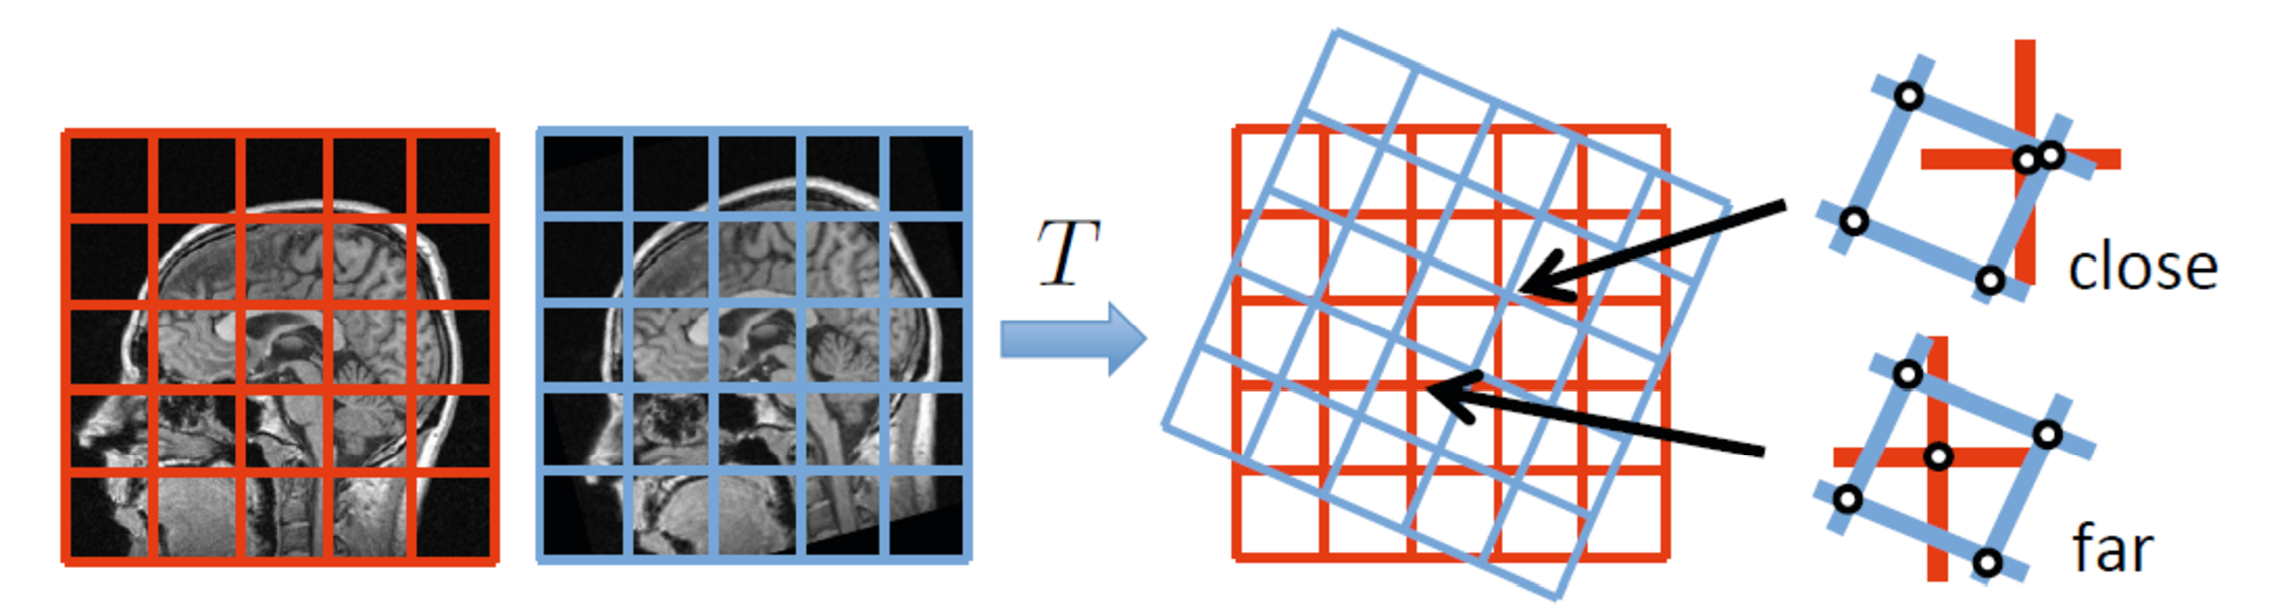
\includegraphics[width=1\linewidth]{Figures/uncertainty_ex}
\end{center}
   \caption{Moving (blue) and fixed (red) images. The interpolation uncertainty varies among grid points after transformations. Above the uncertainty is low because neighbouring points are close in contrary to below where points are far. From \cite{wachinger2014gaussian}.}
\label{fig:uncertainty_ex}
\end{figure}

To have accurate interpolation with prediction of error, a bayesian regression is proposed in this paper. The transformed grid values are the observations and the prediction result in resampled values on the fixed grid. Assuming a $\mathcal{GP}$ prior over images and gaussian noise on the observations, the prediction is gaussian with mean corresponding to resampled values and variance is the uncertainty (sec. \ref{subsec:gpresampling}). This lead to a new similarity measure that takes into account the incertainty of the interpolation (sec. \ref{subsec:sim}). The results of the proposed approach are shown in sec. \ref{sec:exp}, finally the conclusion of this paper summarize the contribution with future perspectives (sec. \ref{sec:concl}).

%-------------------------------------------------------------------------
\section{Method}
\subsection{Gaussian process resampling}\label{subsec:gpresampling}

\begin{equation}
p(I_M^*|I_M;X,X^*)=\mathcal{N}(\mu_{I_M}^*,\Sigma_{I_M}^*)
\end{equation}\label{eq:reg}

\begin{equation}
\mu_{I_M}^*=k(X^*,X).[k(X,X)+\sigma_{I_M}^2\mathbf{I}]^{-1}.I_M
\end{equation}\label{eq:mu}

\begin{equation}
\Sigma_{I_M}^*=k(X^*,X^*)-\frac{\mu_{I_M}^*}{I_M}.k(X,X^*)
\end{equation}\label{eq:sigma}

\begin{equation}
k(\mathbf{x},\mathbf{x'}) =\exp(-\frac{\|{\mathbf{x}-\mathbf{x'}}^2\|}{2l^2})
\end{equation}\label{eq:k}

The method is decomposed into three main steps :
\begin{enumerate}
\item A prediction of the interpolation of the image $J$ is done with a prior gaussian process on the resampled image $J^*$.
\item The optimal registration is generated using a bayesian approach with a multivariate Gaussian Likelihood and the prediction of the gaussian process on $J^*$.
\item Reduction of the computationnal cost for 3D volumes and creation of a new uncertainty estimate (not based on $\mathcal{GP}$) to compare the experiments.
\end{enumerate}

From item 2., they derived a new similarity measure taking into account the uncertainty estimates (thanks to the $\mathcal{GP}$ of item 1.).
Finally, they compare there new similarity with the new interpolation to the gold standard interpolation (NN, linear, spline, cubic).

\subsection{New similarity measure}\label{subsec:sim}

\begin{equation}
p(I_F,I_M,I_M^*)=p(I_M^*|I_M).p(I_F|I_M^*)
\end{equation}\label{eq:joint}

\begin{equation}
p(I_F,I_M,I_M^*)=p(I_M^*|I_M).p(I_F|I_M^*)
\end{equation}\label{eq:joint}

\begin{equation}
\hat{T}=\underset{T}{\textrm{argmax}}~ p(I_F,I_M)
\end{equation}\label{eq:arg}

\begin{equation}
\begin{array} {lcl} 
p(I_F,I_M) & = & \int p(I_F,I_M,I_M^*)~dI_M^*\\ 
& = &  \int p(I_M^*|I_M).p(I_F|I_M^*)~dI_M^*\\
& = &  \int \mathcal{N}(I_M^*;\mu_{I_M}^*,\Sigma_{I_M}^*).\\
&   &  \mathcal{N}(I_F;{I_M}^*,\sigma_{I_F}^2\mathbf{I})~dI_M^*\\
& = &  \mathcal{N}(I_F;\mu_{I_M}^*,\Sigma_{I_M}^*+\sigma_{I_F}^2\mathbf{I})
\end{array}
\end{equation}

\begin{equation}
\begin{array} {lcl} 
\log p(I_F,I_M) &=& \log\big( (2\pi)^{-\frac{k}{2}}|\Sigma|^{-\frac{1}{2}}\big)- \\
 & & \frac{1}{2}(I_F-\mu_{I_M}^*)^t\Sigma^{-1}(I_F-\mu_{I_M}^*)
\end{array}
\end{equation}

\section{Experimentation}\label{sec:exp}

I plan to code and run the program using MATLAB.
After reading and understading all the paper, I will download the database of patent from the available database BrainWeb and RIRE.
I will constrain my work in the registration of 2D images. I will compute the boxplots (with a statistical analysis) to evaluate the impact of the interpolation, the new similarity measure and the gold standard.
To extend their work, it can be interesting to invest other kernels for the $\mathcal{GP}$ and the impacts of its parameters. Maybe the use of an EM algorithm or variationnal bayesian on item 2. can be used to improve the accuracy of the similarity measure.

\section{Conclusion}\label{sec:concl}

{\small
\bibliographystyle{ieee}
\bibliography{egbib}
}

\end{document}
